\documentclass[t]{beamer}

%\documentclass[handout, t]{beamer}
\setbeamertemplate{navigation symbols}{}
\usepackage{pstricks}
\usepackage{mathtools}
\usepackage{amsfonts}
\usepackage{mathrsfs}
\usepackage{amsmath}
\setbeamertemplate{navigation symbols}{}
\usepackage{bm}
\usepackage[UTF8]{ctex}
\usetheme{AnnArbor}
\usefonttheme{serif}
\useinnertheme{rounded}
%\usecolortheme{crane}
\setbeamertemplate{blocks}[rounded][shadow=true]

\newcommand{\dif}{{\;\rm d}}
\usepackage{graphicx}
\usepackage{pgf}
\usepackage{tikz}
\usetikzlibrary{arrows, decorations.pathmorphing, backgrounds, positioning, fit, petri, automata}
\tikzset{>=stealth}

\usepackage{setspace}
\setmainfont{Times New Roman}
\setCJKmainfont{Microsoft YaHei}


\hypersetup{pdfpagemode=FullScreen}
\renewcommand{\Pr}{\mathbb{P}}
\usepackage{blkarray}


\setbeamercolor{block title}{bg=red!10!white}
\setbeamercolor{block body}{bg=gray!10!white}

\usepackage{multicol}
\newcommand{\E}{\mathbb{E}}
\newcommand{\EP}{\mathbb{E}^{\mathbb{P}}}
\newcommand{\EQ}{\mathbb{E}^{\mathbb{Q}}}
\newcommand{\Var}{{\rm Var}}
\newcommand{\Cov}{{\rm Cov}}


\begin{document}
\fontsize{11}{18}\selectfont


\CTEXindent



  \title{第五章~~连续时间马氏链}
\author{随机过程及其在金融中的应用}
\date{中国人民大学出版社}
  \begin{frame}
    \maketitle
  \end{frame}

\begin{frame}{本章内容}
  \begin{multicols}{2}
    \tableofcontents
  \end{multicols}
\end{frame}

\section{定义和例子}

\subsection{连续时间马氏链的概念}
\begin{frame}{连续时间马氏链的概念}
  对于任意状态$i,j,i_0,\ldots,i_{n}$以及任意时间$0\le s_0<s_1<\cdots<s_n<s$,有:
  \[\begin{split}
  \Pr(X_{t+s}=j|X_s=i,X_{s_n}=i_{n},\ldots,X_{s_0}=i_0)&=\Pr(X_{t+s}=j|X_s=i) \\
  &=\Pr(X_{t}=j|X_0=i) \\
  \end{split}\]
  满足上式的就是连续时间马氏链。
  
  从时刻$s$的状态$i$到时刻$(t+s)$的状态$j$的概率,只依赖于时间间隔$t$,而与起始时间$s$无关。

  \begin{block}{注意:}
    在离散时间马氏链中,时间和状态均是离散的。而
  在连续时间马氏链中,{时间是连续的},{状态是离散的}。
  \end{block}
\end{frame}


\begin{frame}{连续时间马氏链的概念(cont.)}

  为了便于区分,离散时间马氏链经过$n$步,从状态$i$转移到状态$j$的概率记作$p^n(i,j)$ (注意:$n$是以上标形式体现),即:
  \[p^n(i,j)=\Pr(X_{t+{n}}=j|X_t=i)=\Pr(X_{n}=j|X_0=i), \qquad n,t \in\mathbb{Z} \]
  而在连续时间马氏链中,
  在$h>0$时间段,从状态$i$转移到状态$j$的概率记作$p_{h}(i,j)$ (注意:$h$是以下标形式体现),即:
  \[p_{h}(i,j)=\Pr(X_{t+{h}}=j|X_t=i)=\Pr(X_{h}=j|X_0=i), \qquad h,t\in\mathbb{R}^+ \]
  此处的连续时间马氏链仍然假设其具有时间齐次性。
\end{frame}

\subsection{连续时间马氏链的性质}
\begin{frame}{连续时间马氏链的性质}
  \begin{block}{连续时间马氏链的C-K方程:}
    \[\sum_k p_s(i,k)p_t(k,j)=p_{s+t}(i,j) \]
  \end{block}
  \begin{center}
    \begin{tikzpicture}[>=stealth, scale=0.8]
    \node [circle](A) at (0,0) {$i$};
    \node [circle](B) at (4,0) {$k$};
    \node [circle](C) at (10,0) {$j$};
    \node at (-1,0) {状态};
    \node at (-1,-.75) {时刻};
    \node at (-1,-1.5) {时间段};
    \draw [->, very thick] (A)--(B) ;
    \draw [->, very thick] (B)--(C) ;
    \node  at (0,-0.75) {$0$};
    \node  at (4,-0.75) {$s$};
    \node  at (10,-0.75) {$s+t$};
    \draw [|<->|, very thick] (0,-1.5)--(4,-1.5) ;
    \draw [|<->|, very thick] (4,-1.5)--(10,-1.5) ;
    \node  at (2,-1.2) {$s$};
    \node  at (7,-1.2) {$t$};
    \end{tikzpicture}
      \end{center}

  与离散时间马氏链类似,由连续时间马氏链的C-K方程也可以得到如下不等式:
  \begin{equation*}
  p_{s+t}(i,j)\ge p_s(i,k)\cdot p_t(k,j), \qquad \forall k
  \end{equation*}

\end{frame}

\begin{frame}{连续时间马氏链的相关定理}
\begin{itemize}
  \item 假设$T_i$是连续时间马氏链停留在状态$i$的时长,则$T_i$服从指数分布。
  \item 对于连续时间马氏链,若对于某个$t>0$,有$p_t(i,j)>0$,则对任意$s>0$,均有$p_{t+s}(i,j)>0$。
\end{itemize}
    
连续时间马氏链中的所有状态均是非周期的,因此无须考虑周期性。
\end{frame}

\subsection{转移速率}
\begin{frame}{转移速率}
  当${h}\to 0$时,引入{转移速率} $q(i,j)$,即:
  \[q(i,j)=\lim_{h\to 0}\frac{p_{h}(i,j)}{h}=\lim_{h\to 0}\frac{\Pr(X_{t+{h}}=j|X_t=i)}{h} \]
  其中,$q(i,j)$表示从状态$i$跳到$j$的转移速率。

  在连续时间马氏链中,除了要考虑某一时刻马氏链处于{什么状态}以外,还要关心它在离开这个状态之前会停留{多长时间}。前面已经证明了这个停留时间具备无记忆性,服从{指数分布}。

通常在连续时间下,通过转移速率来描述系统更为简单。 
\end{frame}

\begin{frame}{转移速率$q(i,j)$的性质}
  \begin{enumerate}
    \item $q(i,i)\le 0,\qquad i=1,2,\ldots,N$
    \item $q(i,j)\ge 0,\; i\ne j,\qquad i,j=1,2,\ldots,N$
    \item $\sum^N_{j=1}q(i,j)=0,\qquad i=1,2,\ldots,N$
  \end{enumerate}

  由于状态间的转移是发生在状态空间内,因此总的转移速率应当为零。这就如同一个封闭容器中水的总量不变,若水从A处流向B处的流速为$x$,则意味着由B处流向A处的流速为$-x$,流速之和仍然为零。

如果转移速率$q(i,j)$对任意状态$j$均满足$q(i,j)=0$,则称状态$i$是吸收态。此时的转移速率均为零,对应到转移速率矩阵上,体现为状态$i$一行的元素取值均为零,说明马氏链将永远停留在状态$i$处。
\end{frame}


\begin{frame}{转移速率矩阵}
  \[{\bf Q}=\begin{bmatrix}
    q(1,1) & q(1,2) & \cdots & q(1,N)\\
    q(2,1) & q(2,2) & \cdots & q(2,N)\\
    \vdots & \vdots &  & \vdots\\
    q(N,1) & q(N,2) & \cdots & q(N,N)\\
    \end{bmatrix} \]
    
    需要注意的是,由于转移速率矩阵每行元素之和等于零,因此该矩阵对角线上的元素$q(i,i)$的绝对值应当等于该行其他元素之和,即:
    \[|q(i,i)|=\sum_{k\ne i}q(i,k),\qquad \forall i \]
    记$q_i=|q(i,i)|=-q(i,i)$,这里的$q_i$就是离开状态$i$的速率。
    
\end{frame}

\subsection{连续时间马氏链的例子}
\begin{frame}{举例1:泊松过程}
  $N(t)$表示速率为$\lambda$的泊松过程到时刻$t$为止的到达数。 
  对于任意时间段$h$,到达数由$n$增加到$(n+1)$的概率为:
  \[\begin{split}
  p_h(n,n+1)&=\frac{(\lambda h)^1}{1!}{\rm e}^{-\lambda h}=\lambda h {\rm e}^{-\lambda h}\\
  &=\lambda h \left[1-\lambda h+\frac{1}{2}(\lambda h)^2-\frac{1}{3!}(\lambda h)^3+\cdots \right]
  \end{split} \]
  因此:
  \[\begin{split}
  q(n,n+1)&=\lim_{h\to 0}\frac{p_h(n,n+1)}{h}\\
  &=\lim_{h\to 0}\lambda \left[1-\lambda h+\frac{1}{2}(\lambda h)^2-\frac{1}{3!}(\lambda h)^3+\cdots \right]=\lambda
  \end{split} \]
  
\end{frame}


\begin{frame}{泊松过程(cont.)}
  在时间$h$内至少经历两步转移的概率为:
  \[\begin{split}
  \Pr[N(t+h)&\ge n+2|N(t)=n]= 1-[p_h(n,n)+p_h(n,n+1)]
  \\&=1-\left( {\rm e}^{-\lambda h}+\lambda h{\rm e}^{-\lambda h}\right)=1-(1+\lambda h){\rm e}^{-\lambda h}  \\
  &=1-(1+\lambda h)\left[1-\lambda h+\frac{1}{2}(\lambda h)^2-\frac{1}{3!}(\lambda h)^3+\cdots  \right]\\
  \end{split} \]
  因此:
\[\frac{\Pr[N(t+h)\ge n+2|N(t)=n]}{h}=\frac{1}{2}\lambda^2 h+\frac{1}{3}\lambda^3 h^2+\cdots \]
\[\lim_{h\to 0}\frac{\Pr[N(t+h)\ge n+2|N(t)=n]}{h}=o(h) \]
从而:$$q(n,n+k)=0,\qquad k\ge 2$$
\end{frame}

\begin{frame}{泊松过程(cont.)}
  因此,在到达发生的速率为$\lambda$的泊松过程中,到达数$N(t)$由$n$增加到$(n+1)$的速率为$\lambda$,其余情形下超过两步的转移速率为0,即:
  \begin{equation*}
  \begin{cases}
  q(n,n+1)=\lambda,\\
  q(n,n+k)=0, & k\ge 2
  \end{cases}\qquad  \forall n\ge0
  \end{equation*}
  相应的转移速率矩阵${\bf Q}$如下:
  \[{\bf Q}=\begin{bmatrix}
  -\lambda & \lambda & 0& 0& \cdots \\
  0& -\lambda & \lambda&0& \cdots\\
  0&0& -\lambda &\lambda& \cdots \\
  0&0& 0 &-\lambda& \cdots \\
  \vdots & \vdots &\vdots &\vdots&\ddots \\
  \end{bmatrix} \]
\end{frame}



\begin{frame}{泊松过程的转移速率图}
  \begin{equation*}
    \begin{cases}
    q(n,n+1)=\lambda,\\
    q(n,n+k)=0, & k\ge 2
    \end{cases}\qquad  \forall n\ge0
    \end{equation*}
  \centering
  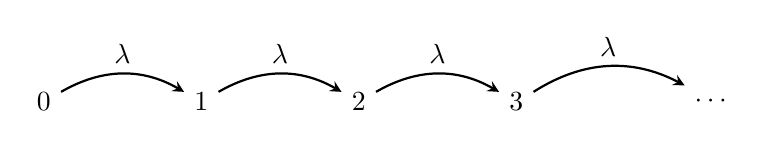
\begin{tikzpicture}[>=stealth, thick]
  \node	(S0) 	at 	(0,0)  	{0};
  \node	(S1)	 at 	(2,0)	 {1};
  \node	(S2)	 at 	(4,0) 	{2};
  \node	(S3)	 at 	(6,0)	 {3};
  \node	(S4)	 at 	(8.5,0) 	{$\cdots$};
  \draw[->](S0)  to [bend left=30] node[auto]{$\lambda$}  (S1) ;
  \draw[->](S1) to [bend left=30] node[auto]{$\lambda$} (S2) ;
  \draw[->](S2) to [bend left=30] node[auto]{$\lambda$} (S3) ;
  \draw[->](S3) to [bend left=30] node[auto]{$\lambda$} (S4) ;
  \end{tikzpicture}

  \begin{block}{说明:}
泊松过程属于计数过程,因此$m>n$时,$q(m,n)=0$。
  \end{block}
\end{frame}

\begin{frame}{举例2:生灭过程}
  在状态空间为$\{0,1,2,\ldots,N\}$的生灭过程(birth-and-death process)中,出生率为$\lambda_n$,死亡率为$\mu_n$,因此有:
  \[\begin{split}
  q(n,n+1)&=\lambda_n, \qquad  n=0,1,2,\ldots, N-1\\
  q(n,n-1)&=\mu_n,\; \qquad n=1,2,\ldots, N
  \end{split} \]
  相应的转移速率矩阵${\bf Q}$如下:\small
  {\[{\bf Q}=\begin{bmatrix}
  -\lambda_0 & \lambda_0 & 0&0 &\cdots &0&0\\
  \mu_1& -(\lambda_1+\mu_1) & \lambda_1&0&\cdots &0&0\\
  0&\mu_2 & -(\lambda_2+\mu_2) &\lambda_2 &\cdots &0&0\\
  \vdots & \vdots &\vdots &\vdots &\ddots & \vdots&\vdots\\
  0&0&0&0&\mu_{N-1} &-(\lambda_{N-1}+\mu_{N-1})&\lambda_{N-1}\\
  0&0&0&0&\cdots& \mu_N &-\mu_N
  \end{bmatrix} \]}
\end{frame}


\begin{frame}{生灭过程的转移速率图}
  \[\begin{cases}
    q(n,n+1)=\lambda_n, &n=0,1,2,\ldots, N-1\\
    q(n,n-1)=\mu_n, &n=1,2,\ldots, N
    \end{cases} \]

    \centering
    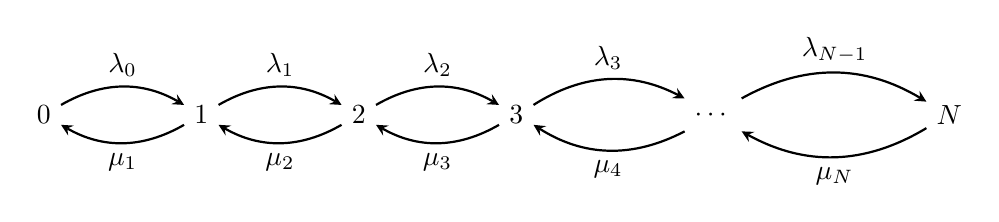
\begin{tikzpicture}[>=stealth, thick]
    \node	(S0) 	at 	(0,0)  	{0};
    \node	(S1)	 at 	(2,0)	 {1};
    \node	(S2)	 at 	(4,0) 	{2};
    \node	(S3)	 at 	(6,0)	 {3};
    \node	(S4)	 at 	(8.5,0) 	{$\cdots$};
    \node	(S5)	 at 	(11.5,0) 	{$N$};
    \draw[->](S0)  to [bend left=30] node[auto]{$\lambda_0$}  (S1) ;
    \draw[->](S1) to [bend right=-30] node[auto]{$\mu_1$} (S0) ;
    
    \draw[->](S1) to [bend left=30] node[auto]{$\lambda_1$} (S2) ;
    \draw[->](S2) to [bend right=-30] node[auto]{$\mu_2$} (S1) ;
    
    \draw[->](S2) to [bend left=30] node[auto]{$\lambda_2$} (S3) ;
    \draw[->](S3) to [bend right=-30] node[auto]{$\mu_3$} (S2) ;
    
    \draw[->](S3) to [bend left=30] node[auto]{$\lambda_3$} (S4) ;
    \draw[->](S4) to [bend right=-30] node[auto]{$\mu_4$} (S3) ;
  
    \draw[->](S4) to [bend left=30] node[auto]{$\lambda_{N-1}$} (S5) ;
  \draw[->](S5) to [bend right=-30] node[auto]{$\mu_N$} (S4) ;
    \end{tikzpicture}
\end{frame}

\begin{frame}{举例3:纯生过程}
  当$\mu=0$时,生灭过程称为纯生过程(pure-birth process)。
  \[\begin{split}
  q(n,n+1)&=\lambda_n, \qquad  n=0,1,2,\ldots\\
  q(n,n-1)&=0,\; \qquad n=1,2,\ldots
  \end{split} \]
  相应的转移速率矩阵${\bf Q}$如下:
  {\[{\bf Q}=\begin{bmatrix}
    -\lambda_0 & \lambda_0 & 0&0 &\cdots \\
    0& -\lambda_1 & \lambda_1&0&\cdots \\
    0&0 & -\lambda_2 &\lambda_2 &\cdots \\
    \vdots & \vdots &\vdots &\vdots & \ddots \\
    \end{bmatrix} \]}
\end{frame}


\begin{frame}{纯生过程的转移速率图}
  \centering
	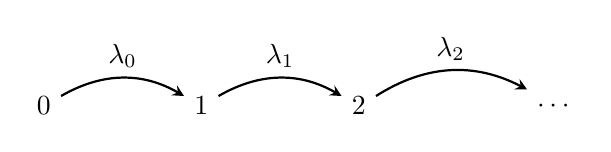
\begin{tikzpicture}[>=stealth, thick]
	
	\node	(S0) 	at 	(0,0)  	{0};
	\node	(S1)	 at 	(2,0)	 {1};
	\node	(S2)	 at 	(4,0) 	{2};
	\node	(S3)	 at 	(6.5,0)	 {$\cdots$};
	\draw[->](S0)  to [bend left=30] node[auto]{$\lambda_0$}  (S1) ;
	\draw[->](S1) to [bend left=30] node[auto]{$\lambda_1$} (S2) ;
	\draw[->](S2) to [bend left=30] node[auto]{$\lambda_2$} (S3) ;
  \end{tikzpicture}
  
  \begin{block}{注意:}
    泊松过程可看作转移速率不变($\lambda_{n}=\lambda$)的纯生过程。
  \end{block}
\end{frame}

\begin{frame}{举例4:$M/M/s$排队系统}
  顾客按速率$\lambda$到达,柜台有$s$个服务窗口,对每个顾客的服务时间相互独立且服从速率为$\mu$的指数分布,因此:
  \[\begin{split}
  q(n,n+1)&=\lambda, \qquad  n=0,1,2,\ldots s-1\\
  q(n,n-1)&=\begin{cases}
  n\mu,& 0\le n\le s\\
  s\mu,& n\ge s
  \end{cases}
  \end{split} \]
  即,当顾客数不多于服务窗口数($n\le s$)时,他们都在接受服务,离开的速率为$n\mu$;当顾客数不少于服务窗口数($n\ge s$)时,所有服务窗口都在工作,离开的速率为$s\mu$。
\end{frame}

\begin{frame}{举例4:$M/M/s$排队系统(cont.)}
  离开速率的这一特点与指数分布的特征有关。指数分布具有如下性质:
  \begin{block}{}
    对于独立同分布的随机变量$\tau_1,\tau_2,\ldots,\tau_n\sim \mathcal{E}(\lambda)$,下式成立:
  \[\tau=\min(\tau_1,\tau_2,\ldots,\tau_n)\sim  \mathcal{E}(n\lambda) \]
  因此,在有$n$位顾客正在接受服务的情况下,最先结束服务离开的时间就是$\tau$,相应的离开速率即为$n\lambda$。
  \end{block}
  

\begin{center}
  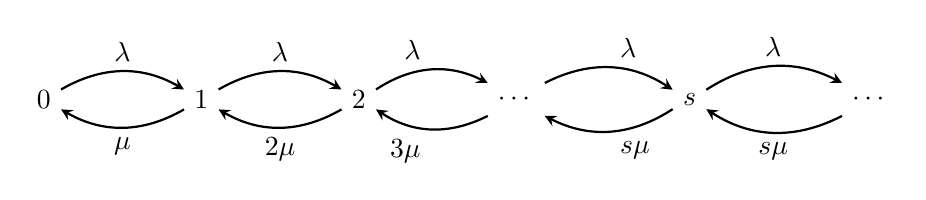
\begin{tikzpicture}[>=stealth, thick]
	
    \node	(S0) 	at 	(0,0)  	{0};
    \node	(S1)	 at 	(2,0)	 {1};
    \node	(S2)	 at 	(4,0) 	{2};
    \node	(S3)	 at 	(6,0)	 {$\cdots$};
    \node	(S4)	 at 	(8.2,0) 	{$s$};
    \node	(S5)	 at 	(10.5,0) 	{$\cdots$};
    \draw[->](S0)  to [bend left=30] node[auto]{$\lambda$}  (S1) ;
    \draw[->](S1) to [bend right=-30] node[auto]{$\mu$} (S0) ;
    
    \draw[->](S1) to [bend left=30] node[auto]{$\lambda$} (S2) ;
    \draw[->](S2) to [bend right=-30] node[auto]{$2\mu$} (S1) ;
    
    \draw[->](S2) to [bend left=30] node[auto]{$\lambda$} (S3) ;
    \draw[->](S3) to [bend right=-30] node[auto]{$3\mu$} (S2) ;
    
    \draw[->](S3) to [bend left=30] node[auto]{$\lambda$} (S4) ;
    \draw[->](S4) to [bend right=-30] node[auto]{$s\mu$} (S3) ;
    
    \draw[->](S4) to [bend left=30] node[auto]{$\lambda$} (S5) ;
    \draw[->](S5) to [bend right=-30] node[auto]{$s\mu$} (S4) ;
    \end{tikzpicture}
\end{center}

\end{frame}


\begin{frame}{举例5:分支过程}
  假设
  每个个体死亡的速率为$\mu$;生育一个新个体的速率为$\lambda$,则有:
  \[q(n,n+1)=n \lambda,\qquad q(n,n-1)=n\mu \]
  \begin{center}
    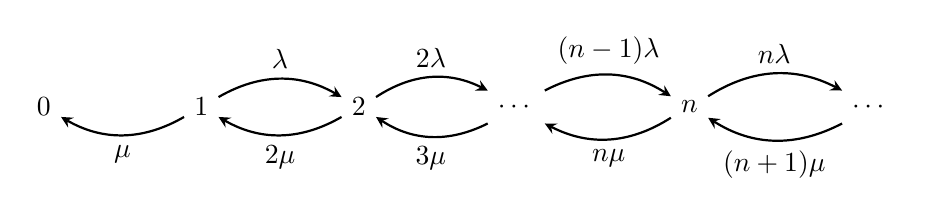
\begin{tikzpicture}[>=stealth, thick]
	
      \node	(S0) 	at 	(0,0)  	{0};
      \node	(S1)	 at 	(2,0)	 {1};
      \node	(S2)	 at 	(4,0) 	{2};
      \node	(S3)	 at 	(6,0)	 {$\cdots$};
      \node	(S4)	 at 	(8.2,0) 	{$n$};
      \node	(S5)	 at 	(10.5,0) 	{$\cdots$};
      \draw[->](S1) to [bend right=-30] node[auto]{$\mu$} (S0) ;
      
      \draw[->](S1) to [bend left=30] node[auto]{$\lambda$} (S2) ;
      \draw[->](S2) to [bend right=-30] node[auto]{$2\mu$} (S1) ;
      
      \draw[->](S2) to [bend left=30] node[above]{$2\lambda$} (S3) ;
      \draw[->](S3) to [bend right=-30] node[below]{$3\mu$} (S2) ;
      
      \draw[->](S3) to [bend left=30] node[above]{$(n-1)\lambda$} (S4) ;
      \draw[->](S4) to [bend right=-30] node[below]{$n\mu$} (S3) ;
      
      \draw[->](S4) to [bend left=30] node[above]{$n\lambda$} (S5) ;
      \draw[->](S5) to [bend right=-30] node[below]{$(n+1)\mu$} (S4) ;
      \end{tikzpicture}
  \end{center}
  
  \begin{block}{说明:}
    当$\mu=0$时,该过程也称为尤尔过程(Yule process)。
  \end{block}
\end{frame}


\section{转移概率}

\subsection{柯尔莫哥洛夫向后方程}
\begin{frame}{柯尔莫哥洛夫向后方程}
  将$[0,t+h]$拆分成$[0,h]$和$[h,t+h]$
\begin{center}
  \begin{tikzpicture}[>=stealth, scale=1.5, thick]
    \node at (0,0){$i$} ;
    \node at (2,0){$k$};
    \node at (5,0){$j$};
    \node at (-1,0){状态};
    \node at (-1,-0.5){时刻};
    \node at (-1,-1){时间段};
    \node at (0,-.5){$0$} ;
    \node at (2,-0.5){$h$};
    \node at (5,-0.5){$t+h$};
    \draw [->](.2,0)--(1.8,0);
    \draw [->] (2.2,0)--(4.8,0);
    \draw [|<->|](0,-1)--(2,-1);
    \draw [|<->|](2,-1)--(5,-1);
    \node at (1,-0.8){$h$} ;
    \node at (3.5,-0.8){$t$};
    \end{tikzpicture}
\end{center}
\[\begin{split}
  p_{t+h}(i,j)-p_t(i,j)&=\left[\sum_kp_h(i,k)p_t(k,j) \right]-p_t(i,j)\\
  &=\left[\sum_{k\ne i}p_h(i,k)p_t(k,j) \right]+\left[p_h(i,i)-1\right]p_t(i,j)
  \end{split}
   \]
   对上式两端同时除以$h$,并令$h\to 0$。
\end{frame}


\begin{frame}{}\small
  \[\begin{split}
    {\lim_{h\to 0}\frac{p_{t+h}(i,j)-p_t(i,j)}{h}}&={\lim_{h\to 0}}\left[{\sum_{k\ne i}\frac{p_h(i,k)}{h}}p_t(k,j) \right]+\left[\lim_{h\to 0}\frac{p_h(i,i)-1}{h}\right]p_t(i,j)\\
    {p'_t(i,j)}&={\sum_{k\ne i}q(i,k)}p_t(k,j)+\left[\lim_{h\to 0}\frac{p_h(i,i)-1}{h}\right]p_t(i,j)
    \end{split}  \]
    注意:
    \[ \lim_{h\to 0}\frac{p_h(i,i)-1}{h}=-\lim_{h\to 0}\sum_{k\ne i}\frac{p_h(i,k)}{h}=-\sum_{k\ne i} q(i,k)=-\lambda_i \]
    因此:
    \[\begin{split}
    p'_t(i,j)&=\sum_{k\ne i}q(i,k)p_t(k,j)-{\left[\lim_{h\to 0}\frac{1-p_h(i,i)}{h}\right]}p_t(i,j)\\
    &=\sum_{k\ne i}q(i,k)p_t(k,j)-{\lambda_i}\; p_t(i,j)\\
    &=\sum_k Q(i,k)p_t(k,j)
    \end{split} \]	\end{frame}


    \begin{frame}{}\small
      \[p'_t(i,j)=\sum_k Q(i,k)p_t(k,j)\]
    其中:
    \[Q(i,k)=\begin{cases}
    q(i,k), & i\ne k\\
    -\lambda_i, & i=k
    \end{cases}\]
    对应的矩阵形式如下:
    \[\begin{bmatrix}
    p'_t(1,1)& \cdots &p'_t(1,n)\\
    p'_t(2,1)& \cdots &p'_t(2,n)\\
    \vdots&  &\vdots\\
    p'_t(n,1)& \cdots &p'_t(n,n)\\
    \end{bmatrix}=
    \begin{bmatrix}
    Q(1,1)& \cdots &Q(1,n)\\
    Q(2,1)& \cdots &Q(2,n)\\
    \vdots&  &\vdots\\
    Q(n,1)& \cdots &Q(n,n)\\
    \end{bmatrix}\begin{bmatrix}
    p_t(1,1)& \cdots &p_t(1,n)\\
    p_t(2,1)& \cdots &p_t(2,n)\\
    \vdots&  &\vdots\\
    p_t(n,1)& \cdots &p_t(n,n)\\
    \end{bmatrix}
     \]
     使用矩阵符号,上式可简写为:
     \[\frac{\dif {\bf P}_t}{\dif t}={\bf Q}{\bf P}_t \]
     该方程称为柯尔莫哥洛夫向后方程(Kolmogorov backward equation),其中${\bf Q}$称作{转移速率矩阵}。在这里将$[0,t+h]$拆分成$[0,h]$和$[h,t+h]$。
\end{frame}

\begin{frame}{举例6:泊松过程的柯尔莫哥洛夫向后方程}
  假设泊松过程的速率为$\lambda$,因此:
  \[q(i,i+1)=\lambda,\qquad q(i,i)=-\lambda \]
  根据
  $p'_t(i,j)=\sum_k Q(i,k)p_t(k,j)$,可得:
  \[\begin{split}
  p'_t(i,j)&=q(i,i+1)p_t(i+1,j)+q(i,i)p_t(i,j)\\
  &=\lambda p_t(i+1,j)-\lambda p_t(i,j)
  \end{split} \]
  假设生灭过程的出生速率为$\lambda_n$,死亡速率为$\mu_n$,因此:
\[q(n,n+1)=\lambda_n,\qquad q(n,n-1)=\mu_n,\qquad q(n,n)=-(\lambda_n+\mu_n) \]
\end{frame}

\begin{frame}{泊松过程的柯尔莫哥洛夫向后方程(cont.)}
根据
$p'_t(n,m)=\sum_k Q(n,k)p_t(k,m)$,可得:
\[\begin{split}
p'_t(n,m)&=q(n,n+1)p_t(n+1,m)+q(n,n-1)p_t(n-1,m)+q(n,n)p_t(n,m)\\
&=\lambda_n p_t(n+1,m)+\mu_n p_t(n-1,m)-(\lambda_n+\mu_n)p_t(n,m)
\end{split} \]	
\end{frame}


\begin{frame}{柯尔莫哥洛夫向前方程}
  如果将$[0,t+h]$拆分成$[0,t]$和$[t,t+h]$,那么得到的方程称为柯尔莫哥洛夫向前方程(Kolmogorov forward equation),使用矩阵符号可以简写为:
  \[\frac{\dif {\bf P}_t}{\dif t}={\bf P}_t {\bf Q}\]
  
\end{frame}


\subsection{转移概率的求解}
\begin{frame}{转移概率的求解}
  根据微分方程的知识,以下方程的通解为$P(t)=C{\rm e}^{at}$:
  \[\frac{\dif P(t)}{\dif t}=aP(t) \]
  在多维情形下也有类似的结论。
  
  由于:
  \[\frac{\dif {\bf P}_t}{\dif t}={\bf Q}{\bf P}_t,\qquad \frac{\dif {\bf P}_t}{\dif t}={\bf P}_t {\bf Q} \]
  因此:
  \begin{equation*}
  {\bf P}_t={\rm e}^{{\bf Q}t}
  \end{equation*}
  其中,${\bf Q}$是转移速率矩阵;${\bf P}_t$是转移概率矩阵。
\end{frame}


\begin{frame}{举例}
  考虑两状态$\{0,1\}$的马氏链,其转移速率矩阵如下:
	\[{\bf Q}=\begin{bmatrix}
	-1&1\\
	2&-2
	\end{bmatrix} \]
	要计算转移概率矩阵${\bf P}_t$,就要求得${\rm e}^{{\bf Q}t}$。
\end{frame}

\begin{frame}{举例(cont.)}
  将矩阵${\bf Q}$对角化:${\bf Q}\to \bm{\Lambda}$,相应地:
	\[{\rm e}^{{\bf Q}t}\to {\rm e}^{\bm{\Lambda}t}={\rm diag}\left( {\rm e}^{\lambda_1 t},{\rm e}^{\lambda_2 t},\ldots,{\rm e}^{\lambda_n t}\right)  \]
	其中,$\bm{\Lambda}={\rm diag}(\lambda_1, \lambda_2,\ldots,\lambda_n)$。
将矩阵${\bf Q}$对角化,其特征值为$0$和$-3$,相应的矩阵可写为:
\[{\bf Q}={\bf X}\bm{\Lambda}{\bf X}^{-1} \]
其中:
\[{\bf X}=\begin{bmatrix}
1&1\\1&-2
\end{bmatrix},\qquad \bm{\Lambda}=\begin{bmatrix}
0&0\\0&-3
\end{bmatrix},\qquad {\bf X}^{-1}=\begin{bmatrix}
\frac{2}{3}&\frac{1}{3}\\\frac{1}{3}&-\frac{1}{3}
\end{bmatrix} \]
\end{frame}

\begin{frame}{举例(cont.)}
相应地:\[\begin{split}
{\bf P}_t&={\rm e}^{{\bf Q}t}={\bf X}{\rm e}^{\bm{\Lambda}t}{\bf X}^{-1}\\
&={\bf X}\begin{bmatrix}
1&0\\
0&{\rm e}^{-3t}
\end{bmatrix}{\bf X}^{-1}=\begin{bmatrix}
\frac{2}{3}&\frac{1}{3}\\\frac{2}{3}&\frac{1}{3}
\end{bmatrix}+{\rm e}^{-3t}\begin{bmatrix}
\frac{1}{3}&-\frac{1}{3}\\-\frac{2}{3}&\frac{2}{3}
\end{bmatrix}\\
\end{split} \]
最终可得转移概率矩阵:
\[\begin{split}
{\bf P}_t={\rm e}^{{\bf Q}t}&=\begin{bmatrix}
\frac{2}{3}&\frac{1}{3}\\\frac{2}{3}&\frac{1}{3}
\end{bmatrix}+{\rm e}^{-3t}\begin{bmatrix}
\frac{1}{3}&-\frac{1}{3}\\-\frac{2}{3}&\frac{2}{3}
\end{bmatrix}\\
&=\begin{bmatrix}
	\frac{2}{3}+\frac{1}{3}{\rm e}^{-3t}&\frac{1}{3}-\frac{1}{3}{\rm e}^{-3t}\\
	\frac{2}{3}-\frac{2}{3}{\rm e}^{-3t}&\frac{1}{3}+\frac{2}{3}{\rm e}^{-3t}
\end{bmatrix}
\end{split}
\]
\end{frame}


\begin{frame}{举例(cont.)}
  \[{\bf P}_t=\begin{bmatrix}
    \frac{2}{3}+\frac{1}{3}{\rm e}^{-3t}&\frac{1}{3}-\frac{1}{3}{\rm e}^{-3t}\\
    \frac{2}{3}-\frac{2}{3}{\rm e}^{-3t}&\frac{1}{3}+\frac{2}{3}{\rm e}^{-3t}
  \end{bmatrix} \]
  当$t\to\infty$时,
  \[\lim_{t\to\infty}{\bf P}_t=\begin{bmatrix}
  \frac{2}{3}&\frac{1}{3}\\\frac{2}{3}&\frac{1}{3}
  \end{bmatrix} \]
  该连续时间马氏链的平稳分布为
\[\pi_1=\frac{2}{3},\qquad 
\pi_2=\frac{1}{3}\]
\end{frame}


\section{极限行为}

\subsection{平稳分布}

\begin{frame}{不可约马氏链}
\begin{block}{定义}
  如果对任意状态$i$和$j$,都有可能从$i$经过有限步转移到$j$,则称马氏链是{不可约}的,即,存在状态序列$k_0=i,\; k_1,\;\ldots,\;k_n=j$,使得$q(k_{m-1},k_m)>0$ $(1\le m\le n)$。
\end{block}

\begin{block}{定理}
  \begin{itemize}
    \item 	如果一个连续时间马氏链$X_t$不可约,且$t>0$,则$p_t(i,j)>0$。
    \item 如果一个连续时间马氏链$X_t$不可约,且具有平稳分布$\bm{\pi}$,则:
    \[\lim_{t\to\infty}p_t(i,j)=\pi(j) \]
  \end{itemize}
\end{block}
\end{frame}


\begin{frame}{平稳分布}
  连续时间马氏链具有非周期性,并且停留时间服从指数分布,因此连续时间马氏链的极限行为比离散时间马氏链更为简单。

  在离散时间下,平稳分布是${\bm\pi}{\bf P}=\bm{\pi}$的一个解;而在连续时间下,对$\forall t>0$,都有${\bm\pi}{\bf P}_t=\bm{\pi}$成立。
但是在实践中,由于${\bf P}_t$不容易计算,因此${\bm\pi}{\bf P}_t=\bm{\pi}$成立的条件难以验证。  

\begin{block}{定理}
    当且仅当$\bm{\pi}{\bf Q}={\bf 0}$时,$\bm{\pi}$是一个平稳分布。
  \end{block}
\end{frame}

\begin{frame}{平稳分布(cont.)}
  \small
  \begin{block}{简单证明}
    由概率平稳性的定义可知:$\bm{\pi}{\bf P}_t=\bm{\pi}$
    ,根据柯尔莫哥洛夫向后方程,有:
    \[\frac{\dif {\bf P}_t}{\dif t}={\bf P}_t{\bf Q} \]
    方程两端同时左乘平稳概率$\bm{\pi}$,可得:
    \[\begin{split}
    \frac{\dif (\bm{\pi}{\bf P}_t)}{\dif t}&=(\bm{\pi}{\bf P}_t){\bf Q}\\
    \frac{\dif\bm{\pi}}{\dif t}&=\bm{\pi}{\bf Q}
    \end{split} \]
    由于平稳概率$\bm{\pi}$与时间$t$无关,因此可得:
    \begin{equation*}
    \bm{\pi}{\bf Q}={\bf 0}	
    \end{equation*}
    \end{block}
\end{frame}


\begin{frame}{举例7:天气链}
  某地的天气有三种状态,分别为晴、雾、雨。已知晴天的持续时间服从均值为3天的指数分布;雾天的持续时间服从均值为4天的指数分布;雨天的持续时间服从均值为1天的指数分布。由此得到的转移速率矩阵如下:
  \[{\bf Q}=  \begin{bmatrix}
  -\frac{1}{3}&\frac{1}{3}&0\\
  0&-\frac{1}{4}&\frac{1}{4}\\
  1 &0&-1
  \end{bmatrix} \]
  求每种天气所占的比例。

  \begin{block}{思路:}
    根据$\bm{\pi}{\bf Q}={\bf 0}$计算。
  \end{block}
\end{frame}

\begin{frame}{天气链(cont.)}
  \[\begin{cases}
    -\frac{1}{3}\pi_1+\pi_3=0\\ 
   \frac{1}{3}\pi_1-\frac{1}{4}\pi_2=0\\ 
   {\frac{1}{4}\pi_2-\pi_3=0}\\
   \pi_1+\pi_2+\pi_3=1
   \end{cases} \Rightarrow\quad \begin{cases}
   \pi_1=0.375\\
   \pi_2=0.5\\
   \pi_3=0.125
   \end{cases} \]
   因此,晴天、雾天和雨天所占的比例分别为37.5\%、50\%和12.5\%。
\end{frame}


\begin{frame}{使用软件求解}
  需要将方程组中的第三个方程删去,可得:
  \[\begin{cases}
   -\frac{1}{3}\pi_1+\pi_3=0\\
  \frac{1}{3}\pi_1-\frac{1}{4}\pi_2=0\\ 
  {\frac{1}{4}\pi_2-\pi_3=0}\\
  \pi_1+\pi_2+\pi_3=1
  \end{cases} \Rightarrow\quad \begin{cases}
   -\frac{1}{3}\pi_1+\pi_3=0\\
  \frac{1}{3}\pi_1-\frac{1}{4}\pi_2=0\\
  \pi_1+\pi_2+\pi_3=1
  \end{cases}\]
  删减后的方程组的矩阵-向量形式如下:
  \[\underbrace{\begin{bmatrix}
    \pi_1&\pi_2&\pi_3
    \end{bmatrix}}_{\bm\pi}\underbrace{\begin{bmatrix}
  	-\frac{1}{3}&\frac{1}{3}&1\\
  	0&-\frac{1}{4}&1\\
    1 &0&1
    \end{bmatrix}}_{\bf A}=\underbrace{\begin{bmatrix}
    0&0&1
    \end{bmatrix}}_{\bf b} \quad \Rightarrow\quad  \bm{\pi}{\bf A}={\bf b} \]
  \end{frame}


  \begin{frame}{使用软件求解(cont.)}
  对矩阵-向量形式的方程进行运算,可得:
  \begin{equation*}
   \bm{\pi}={\bf b}{\bf A}^{-1}
  \end{equation*}
  将数值代入计算,可得:
\[\bm{\pi}={\bf b}{\bf A}^{-1}=\begin{bmatrix}
0&0&1
\end{bmatrix}\begin{bmatrix}
-\frac{1}{3}&\frac{1}{3}&1\\
 0&-\frac{1}{4}&1\\
1 &0&1
\end{bmatrix}^{-1} \]
$\bm{\pi}$的结果刚好就是对应的${\bf A}^{-1}$的最后一行。
\[\bm{\pi}=\begin{bmatrix}
0.375&    0.5&    0.125
\end{bmatrix} \]
\end{frame}

\subsection{细致平衡条件}
\begin{frame}{细致平衡条件}
  连续时间马氏链,若对$\forall j\ne k$,均有:
  \begin{equation*}
    \pi(k)q(k,j)=\pi(j)q(j,k)
  \end{equation*}
  则称$\bm{\pi}$满足细致平衡条件。

  \begin{block}{对比:}
    离散时间马氏链的细致平衡条件:
\begin{equation*}
\pi(k)p(k,j)=\pi(j)p(j,k)
\end{equation*}
  \end{block}
\end{frame}


\begin{frame}{细致平衡条件(cont.)}
  若连续时间马氏链满足细致平衡条件,即:
  \[\pi(k)q(k,j)=\pi(j)q(j,k),\qquad  \forall j\ne k\]
  则${\bm{\pi}}$是一个平稳分布。

  可以根据此定理,利用细致平衡条件,进而求得平稳分布${\bm{\pi}}$,从而不必通过${\bm{\pi}}{\bf Q}={\bf 0}$来求平稳分布。
\end{frame}

\begin{frame}{举例8:生灭链}
  考虑状态空间为$S=\{0,1,\ldots,N\}$的生灭链,其转移速率如下:
  \[\begin{cases}
  q(n,n+1)=\lambda_n,& n<N\\
  q(n,n-1)=\mu_n,& n>0
  \end{cases} \]
  求其平稳分布。
\end{frame}


\begin{frame}{生灭链(cont.)}\small
  根据细致平衡条件,可得:
  \[\begin{split}
  \pi(n)q(n,n+1)&=\pi(n+1)q(n+1,n)\\
  \pi(n)\lambda_n&=\pi(n+1)\mu_{n+1}\\
  \frac{\pi(n+1)}{\pi(n)}&=\frac{\lambda_n}{\mu_{n+1}}
  \end{split} \]
  因此:\[
  \frac{\pi(n+1)}{\pi(n)}\cdot \frac{\pi(n)}{\pi(n-1)}\cdot \cdots\cdot \frac{\pi(1)}{\pi(0)}=\frac{\lambda_n}{\mu_{n+1}}\cdot \frac{\lambda_{n-1}}{\mu_{n}}\cdot \cdots\cdot \frac{\lambda_0}{\mu_{1}}\]
  \[\pi(n+1)=\frac{\lambda_n\cdot \lambda_{n-1}\cdot \cdots\cdot  \lambda_0}{\mu_{n+1}\cdot \mu_n\cdot\cdots\cdot\mu_1}\pi(0)
  \]
  从而:\begin{equation*}
  \pi(n)=\frac{\lambda_{n-1}\cdot \lambda_{n-2}\cdot \cdots\cdot  \lambda_0}{\mu_{n}\cdot \mu_{n-1}\cdot\cdots\cdot\mu_1}\cdot \pi(0),\qquad 0<n<N
  \end{equation*}
  其中,$\pi(n)$是生灭链中状态$n$的平稳概率。	
\end{frame}

\begin{frame}{举例9:$M/M/\infty$排队系统}
  状态$S=\{0,1,\ldots \}$,其转移速率如下:
  \[q(n,n+1)=\lambda,\qquad q(n,n-1)=n\mu \]
  求其平稳分布。

  \begin{block}{思路:}
    $M/M/s$排队系统$(s\to\infty)$可看作生灭过程的特殊形式。
    \[\mu_n=n\mu,\qquad \lambda_0=\lambda_1=\cdots=\lambda \]
  \end{block}
\end{frame}


\begin{frame}{$M/M/\infty$排队系统(cont.)}\small
  根据生灭链的公式可得:
  \[\pi(n)=\frac{\lambda_{n-1}\cdot \lambda_{n-2}\cdot\cdots \cdot\lambda_0}{\mu_{n}\cdot \mu_{n-1}\cdot\cdots\cdot\mu_1}\pi(0)=\frac{\lambda^n}{n!\mu^n}\pi(0)=\frac{(\lambda/\mu)^n}{n!}\pi(0)\]
  
  进一步地,由于概率要满足完备性,因此:
  \[\sum_{n=0}^{\infty} \pi(n)=\sum_{n=0}^{\infty}\frac{\lambda^n}{n!\mu^n}\pi(0)=\pi(0)\cdot \sum_{n=0}^{\infty} \frac{(\lambda/\mu)^n}{n!}=1 \]
  因此:$$\pi(0)={\rm e}^{-\lambda/\mu}$$ 最终可得:
  \[\pi(n)=\frac{(\lambda/\mu)^n}{n!}\cdot {\rm e}^{-\lambda/\mu}\]
  由此可见,$M/M/\infty$排队系统的平稳分布$\bm{\pi}$服从均值为$\lambda/\mu$的泊松分布。
\end{frame}

\begin{frame}{举例10:理发店问题}
  理发店一名理发师理发的速率为3(这里以每小时的顾客数为单位,即每位
  顾客的理发时间服从均值为20分钟的指数分布),假设顾客按照一个速率为2的泊松过
  程到达,但是,如果顾客到达时等候室的两把椅子都已坐满,那么他将离开。
  
  求其平稳分布。

\begin{block}{思路:转移速率图}
  \centering
  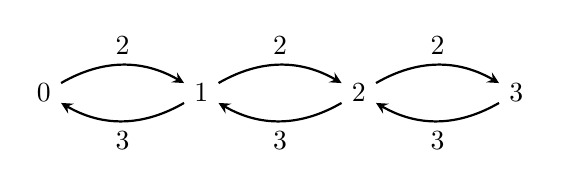
\begin{tikzpicture}[>=stealth, thick]
	
    \node	(S0) 	at 	(0,0)  	{0};
    \node	(S1)	 at 	(2,0)	 {1};
    \node	(S2)	 at 	(4,0) 	{2};
    \node	(S3)	 at 	(6,0)	 {3};
    \draw[->](S0) to [bend right=-30] node[auto]{2} (S1) ;
    \draw[->](S1) to [bend right=-30] node[auto]{3} (S0) ;
    
    \draw[->](S1) to [bend left=30] node[auto]{2} (S2) ;
    \draw[->](S2) to [bend right=-30] node[auto]{3} (S1) ;
    
    \draw[->](S2) to [bend left=30] node[above]{2} (S3) ;
    \draw[->](S3) to [bend right=-30] node[below]{3} (S2) ;
    \end{tikzpicture}
\end{block}

\end{frame}


\begin{frame}{理发店问题(cont.)}
  该问题中的
  状态空间$S=\{0,1,2,3\}$,其对应的转移速率如下:
  \[\begin{cases}
  q(n,n+1)=2,& n=0,1,2\\
  q(n,n-1)=3,& n=1,2,3
  \end{cases} \]	
  
  根据细致平衡条件$\pi(n)q(n,n+1)=\pi(n+1)q(n+1,n)$,有:
  \[\begin{cases}
  \pi(0)q(0,1)=\pi(1)q(1,0)\\
  \pi(1)q(0,2)=\pi(2)q(2,1)\\
  \pi(2)q(0,3)=\pi(3)q(3,2)\\
  \end{cases} \Rightarrow\quad 
  \begin{cases}
  2\pi(0)=3\pi(1)\\
  2\pi(1)=3\pi(2)\\
  2\pi(2)=3\pi(3)
  \end{cases} \]
  结合$\pi(0)+\pi(1)+\pi(2)+\pi(3)=1$,可得:
  \[\pi(0)=\frac{27}{65},\quad \pi(1)=\frac{18}{65},\quad \pi(2)=\frac{12}{65},\quad \pi(3)=\frac{8}{65} \]
  
\end{frame}

\begin{frame}{理发店问题(cont.)}\small
  若采用${\bm{\pi}}{\bf Q}={\bf 0}$求解,过程如下:
  \[{\bf Q}=\begin{bmatrix}
  -2 & 2 & 0&0\\
  3&-5&2&0\\
  0&3&-5&2\\
  0&0&3&-3
  \end{bmatrix} \]
  从而得到:
  \[\begin{cases}
  -2\pi_0+3\pi_1=0\\
  2\pi_0-5\pi_1+3\pi_2=0\\
  2\pi_1-5\pi_2+3\pi_3=0\\
  2\pi_2-3\pi_3=0\\
  \pi_0+\pi_1+\pi_2+\pi_3=1
  \end{cases}\Rightarrow\quad 
  \begin{cases}
   \pi_0=\frac{27}{65}\\
   \pi_1=\frac{18}{65}\\
   \pi_2=\frac{12}{65}\\
  \pi_3=\frac{8}{65}\\
  \end{cases}
  \]	
\end{frame}

\section{嵌入链}

\subsection{嵌入链的概念及特征}

\begin{frame}{嵌入链}
  嵌入链(embedded chain)是对连续时间马氏链的另一种描述方式。

  \begin{block}{定义}
    对于转移速率矩阵为$\bf Q$的连续时间马氏链而言,满足如下条件的$r(i,j)$所构成的就是对应的嵌入链。
\begin{equation*}
r(i,j)=\begin{cases}
\dfrac{q(i,j)}{\sum_{i\ne j}q(i,j) }= \dfrac{q(i,j)}{q(i)},& i\ne j\\
0,& i=j
\end{cases}
\end{equation*}
其中,$q(i,j)$是转移速率矩阵$\bf Q$的对应元素,$q(i)$是离开状态$i$的速率,并且$q(i)=-q(i,i)$。
  \end{block}
\end{frame}

\begin{frame}{理发店问题回顾}
  状态空间$S=\{0,1,2,3\}$对应的转移速率矩阵$\bf Q$如下:
  \begin{equation*}
  {\bf Q}=\begin{bmatrix}
  -2 & 2 & 0&0\\
  3&-5&2&0\\
  0&3&-5&2\\
  0&0&3&-3
  \end{bmatrix}
  \end{equation*}
  根据嵌入链的定义,可以得到对应的嵌入链转移概率矩阵$\bf R$如下:
  \begin{equation*}
  {\bf R}=\begin{bmatrix}
  0 & 1 & 0&0\\
\frac{3}{5}&0&\frac{2}{5}&0\\
0&\frac{3}{5}&0&\frac{2}{5}\\
  0&0&1&0
  \end{bmatrix}
  \end{equation*}
\end{frame}

\begin{frame}{理发店问题(cont.)}
  \begin{equation*}
    {\bf R}=\begin{bmatrix}
    0 & 1 & 0&0\\
  \frac{3}{5}&0&\frac{2}{5}&0\\
  0&\frac{3}{5}&0&\frac{2}{5}\\
    0&0&1&0
    \end{bmatrix}
    \end{equation*}

    这个矩阵反映了由状态$i$转移到可能的状态$j$的概率。该矩阵的主对角线元素均为零,说明嵌入链的转移概率不考虑状态在原地不变的情形。

    \begin{block}{注意:}
      这里转移概率的取值是假设转移服从速率为$q(i,j)$的指数分布,并利用指数分布的性质得到的。
    \end{block}
\end{frame}


\begin{frame}{理发店问题(cont.)}
  \begin{equation*}
    {\bf Q}=\begin{bmatrix}
      -2 & 2 & 0&0\\
      3&-5&2&0\\
      0&3&-5&2\\
      0&0&3&-3
      \end{bmatrix}\quad  {\bf R}=\begin{bmatrix}
    0 & 1 & 0&0\\
  \frac{3}{5}&0&\frac{2}{5}&0\\
  0&\frac{3}{5}&0&\frac{2}{5}\\
    0&0&1&0
    \end{bmatrix}
    \end{equation*}
    从状态1转移到状态0的速率为3,转移到状态2的速率为2,因此从状态1首先转移到状态0的概率为:
    \begin{equation*}
    \Pr(X_{\tau}=0|X_0=1)=\Pr[T_1=\min(T_1,T_2)]=\frac{3}{2+3}=\frac{3}{5}
    \end{equation*}
    类似地,从状态1首先转移到状态2的概率为:
    \begin{equation*}
    \Pr(X_{\tau}=2|X_0=1)=\Pr[T_2=\min(T_1,T_2)]=\frac{2}{2+3}=\frac{2}{5}
    \end{equation*}
  
\end{frame}


\begin{frame}{泊松过程的嵌入链}\small
  对于泊松过程,其转移速率满足$q(i,i+1)=\lambda$,并且$q(i,i)=-\lambda$,因此:
\[r(i,i)=0,\qquad r(i,i+1)=1 \]
相应的转移速率矩阵与嵌入链的转移概率矩阵分别如下:
\[{\bf Q}=\begin{bmatrix}
-\lambda & \lambda&0&0&0&0&\cdots\\
0&-\lambda & \lambda&0&0&0&\cdots\\
0&0&-\lambda & \lambda&0&0&\cdots\\
0&0&0&-\lambda & \lambda&0&\cdots\\
0&0&0&0&-\lambda & \lambda&\cdots\\
\vdots &\vdots&\vdots&\vdots&\vdots&\vdots&\ddots
\end{bmatrix} \qquad 
{\bf R}=\begin{bmatrix}
0 & 1&0&0&0&0&\cdots\\
0&0 & 1&0&0&0&\cdots\\
0&0&0 & 1&0&0&\cdots\\
0&0&0&0 & 1&0&\cdots\\
0&0&0&0&0 &1&\cdots\\
\vdots &\vdots&\vdots&\vdots&\vdots&\vdots&\ddots
\end{bmatrix}\]
\end{frame}


\begin{frame}{有吸收态的嵌入链}\small
  \[{\bf Q}=\begin{bmatrix}
    0&0&0&0&0\\
    10&-20&10&0&0\\
    0&10&-30&20&0\\
    0&0&10&-40&30\\
    0&0&0&0&0\\
      \end{bmatrix}\]
    对于有吸收态$i$的连续时间马氏链,$q(i,i)=0$。同时,与之对应的嵌入链转移概率$r(i,i)=1$。
    
    上面的转移速率矩阵${\bf Q}$有两个吸收态1和5。于是对应的嵌入链转移概率矩阵${\bf R}$如下:
    \[ 	{\bf R}=\begin{bmatrix}
    1&0&0&0&0\\
    1/2&0&1/2&0&0\\
    0&1/3&0&2/3&0\\
    0&0&1/4&0&3/4\\
    0&0&0&0&1\\
      \end{bmatrix}\]
\end{frame}


\begin{frame}{嵌入链转移概率的特点}
  嵌入链的转移概率与连续时间马氏链的转移概率的不同之处在于,前者并未考虑时间因素,只关心状态与状态之间的转移概率。
\end{frame}


\subsection{利用嵌入链计算平稳分布}
\begin{frame}{嵌入链}\small
  根据${\bm{\pi}}{\bf Q}={\bf 0}$可得:
\begin{equation*}
\sum_i \pi(i)q(i,j)=0\quad \Rightarrow\quad \sum_{i\ne j} \pi(i)q(i,j)=\pi(j)q(j)
\end{equation*}
定义$\psi(i)=\pi(i)q(i)$,将其分别代入上式的左右两侧,可得:
\[\begin{cases}
 \sum_{i\ne j} \pi(i)q(i,j)=\sum_{i\ne j} \psi(i)\frac{q(i,j)}{q(i)}=\sum_{i\ne j} \psi(i)r(i,j)\\
\pi(j)q(j)=\psi(j)
\end{cases}\]
因此:
\begin{equation*}
\psi(j)=\sum_{i\ne j} \psi(i)r(i,j)
\end{equation*}
其中,$r(i,j)$是嵌入链对应的转移概率,反映了连续时间马氏链状态之间转移的概率。
\end{frame}


\begin{frame}{矩阵-向量形式}
\[\psi(j)=\sum_{i\ne j} \psi(i)r(i,j)
\]
上式的矩阵-向量形式如下:
  \begin{equation*}
\bm{\psi}{\bf R}=\bm{\psi}
\end{equation*}
其中,$\bm{\psi}$是嵌入链的平稳分布。

\begin{block}{注意:}
  可根据该性质,通过嵌入链${\bf R}$计算连续时间马氏链的平稳分布$\bm{\pi}$。
\end{block}

\end{frame}


\begin{frame}{通过嵌入链计算平稳分布的具体步骤}\small
  \begin{itemize}
    \item 基于嵌入链$\bf R$,利用$\bm{\psi}{\bf R}=\bm{\psi}$计算出嵌入链的平稳分布$\bm{\psi}$:
	$$\bm{\psi}=\begin{bmatrix}
	\psi(1) & \psi(2) & \cdots & \psi(n)
  \end{bmatrix}$$
  \item 将得到的嵌入链平稳分布中的各元素分别除以对应的转移速率矩阵主对角线元素的绝对值,即$\psi(i)/q(i)$,从而得到向量$\widetilde{\bm{\pi}}$,即:
	\[\widetilde{\bm{\pi}}=\begin{bmatrix}
		\frac{\psi(1)}{q(1)} & \frac{\psi(2)}{q(2)} & \cdots & \frac{\psi(n)}{q(n)}
	\end{bmatrix} \]

  \item 最后对向量$\widetilde{\bm{\pi}}$进行归一化(normalize)操作,得到连续时间马氏链的平稳分布$\bm{\pi}$,即:
	\[\bm{\pi}=\frac{1}{A}\widetilde{\bm{\pi}}=\frac{1}{A}\begin{bmatrix}
		\frac{\psi(1)}{q(1)} & \frac{\psi(2)}{q(2)} & \cdots & \frac{\psi(n)}{q(n)}
	\end{bmatrix} \]	
	其中,$A$是归一化因子,并且$A=\sum_{k=1}^{n}\frac{\psi(k)}{q(k)}$。

  \end{itemize}

\end{frame}


\begin{frame}{$\pi(i)$与$\psi(i)$的关系}
  连续时间马氏链的平稳分布概率$\pi(i)$衡量的是,长期看来过程花费在状态$i$上的时间占总时间的比重;而嵌入链的平稳分布概率$\psi(i)$衡量的则是,长期看来转移至状态$i$的次数占总的转移次数的比重。
  
  简言之,$\bm{\pi}$关注花费在各状态上的时间所占的比重;$\bm{\psi}$关注各状态转移的次数所占的比重。
\end{frame}


\begin{frame}{举例:}
  考虑一个三状态连续时间马氏链,其转移速率矩阵如下:
	\[{\bf Q}=\begin{bmatrix}
	-2 & 1 &1\\
	2 & -4 &2\\
	4 & 4 &-8\\
	\end{bmatrix} \]
	求该链的平稳分布$\bm{\pi}$。
\end{frame}




\begin{frame}{解法一}
  使用${\bm{\pi}}{\bf Q}={\bf 0}$来求解,可以列出如下方程组:
	\[\begin{cases}
	-2\pi(1)+2\pi(2)+4\pi(3)=0\\
	\pi(1)-4\pi(2)+4\pi(3)=0\\
	\pi(1)+\pi(2)+\pi(3)=1
	\end{cases}\Rightarrow\quad \begin{cases}
	\pi(1)=\frac{4}{7}\\
 	\pi(2)=\frac{2}{7}\\
	\pi(3)=\frac{1}{7}\\
	\end{cases} \]
\end{frame}


\begin{frame}{解法二}
  由转移速率矩阵${\bf Q}$,可得到对应的嵌入链${\bf R}$。
	\[{\bf R}=\begin{bmatrix}
	0 & 0.5 & 0.5\\
	0.5 & 0 & 0.5\\
	0.5 & 0.5 & 0\\
	\end{bmatrix} \]
	由于该链是一个双随机链,因此:$$\bm{\psi}=\begin{bmatrix}
	\dfrac{1}{3}&\dfrac{1}{3}&\dfrac{1}{3}
	\end{bmatrix}$$
从而:
	\[\widetilde{\bm{\pi}}=\begin{bmatrix}
	\dfrac{\psi(1)}{q(1)} & \dfrac{\psi(2)}{q(2)} & \dfrac{\psi(3)}{q(3)}
	\end{bmatrix}=\begin{bmatrix}
		\dfrac{1/3}{2}&\dfrac{1/3}{4}&\dfrac{1/3}{8}
	\end{bmatrix}=\begin{bmatrix}
		\dfrac{1}{6} & \dfrac{1}{12} & \dfrac{1}{24}
  \end{bmatrix} \]
\end{frame}


\begin{frame}{解法二(cont.)}
  相应的归一化因子为:
	\[A= \frac{1}{6}+\frac{1}{12}+\frac{1}{24}=\frac{7}{24} \]
	因此:
	\[\bm{\pi}=\frac{1}{A}\widetilde{\bm{\pi}}=\frac{24}{7}\begin{bmatrix}
		\dfrac{1}{6} & \dfrac{1}{12} & \dfrac{1}{24}
		\end{bmatrix}=\begin{bmatrix}
		\dfrac{4}{7} & \dfrac{2}{7} & \dfrac{1}{7}
		\end{bmatrix} \]
	不难看出,两种解法得到的结果完全相同。
\end{frame}






\end{document}